\chapter{系统的功能测试}
\section{设备添加到系统管理表}
	查看当前的驱动程序是否已经添加到了系统当中,我们自定义的cp210xDevRead()、cp210xDevWrite()、cp210xDevOpen()、cp210xDevClose()、cp210xDevIoctl()是否已经和被注册到了IO子系统当中。只有成功的注册到了IO子系统当中,应用层的软件才能够通过标准接口open()、close()、read()、write()、ioctl()来对设备进行操作,完成设备的功能。
	首先通过iosDrvShow查看当前的cp210xDrvInit是否已经将驱动程序接口添加到了驱动程序列表当中,驱动加载前的系统设备表如\autoref{fig:iosDevShow}所示,驱动加载后的系统设备表如\autoref{fig:加载驱动后系统上的设备表}所示,显示了加载了驱动驱动之后多出来了一个驱动号为14的设备。由于两种情况下进行为不同的设备命名策略,所以显示出两个不一样的设备名。
\begin{figure}[!h]
\centering
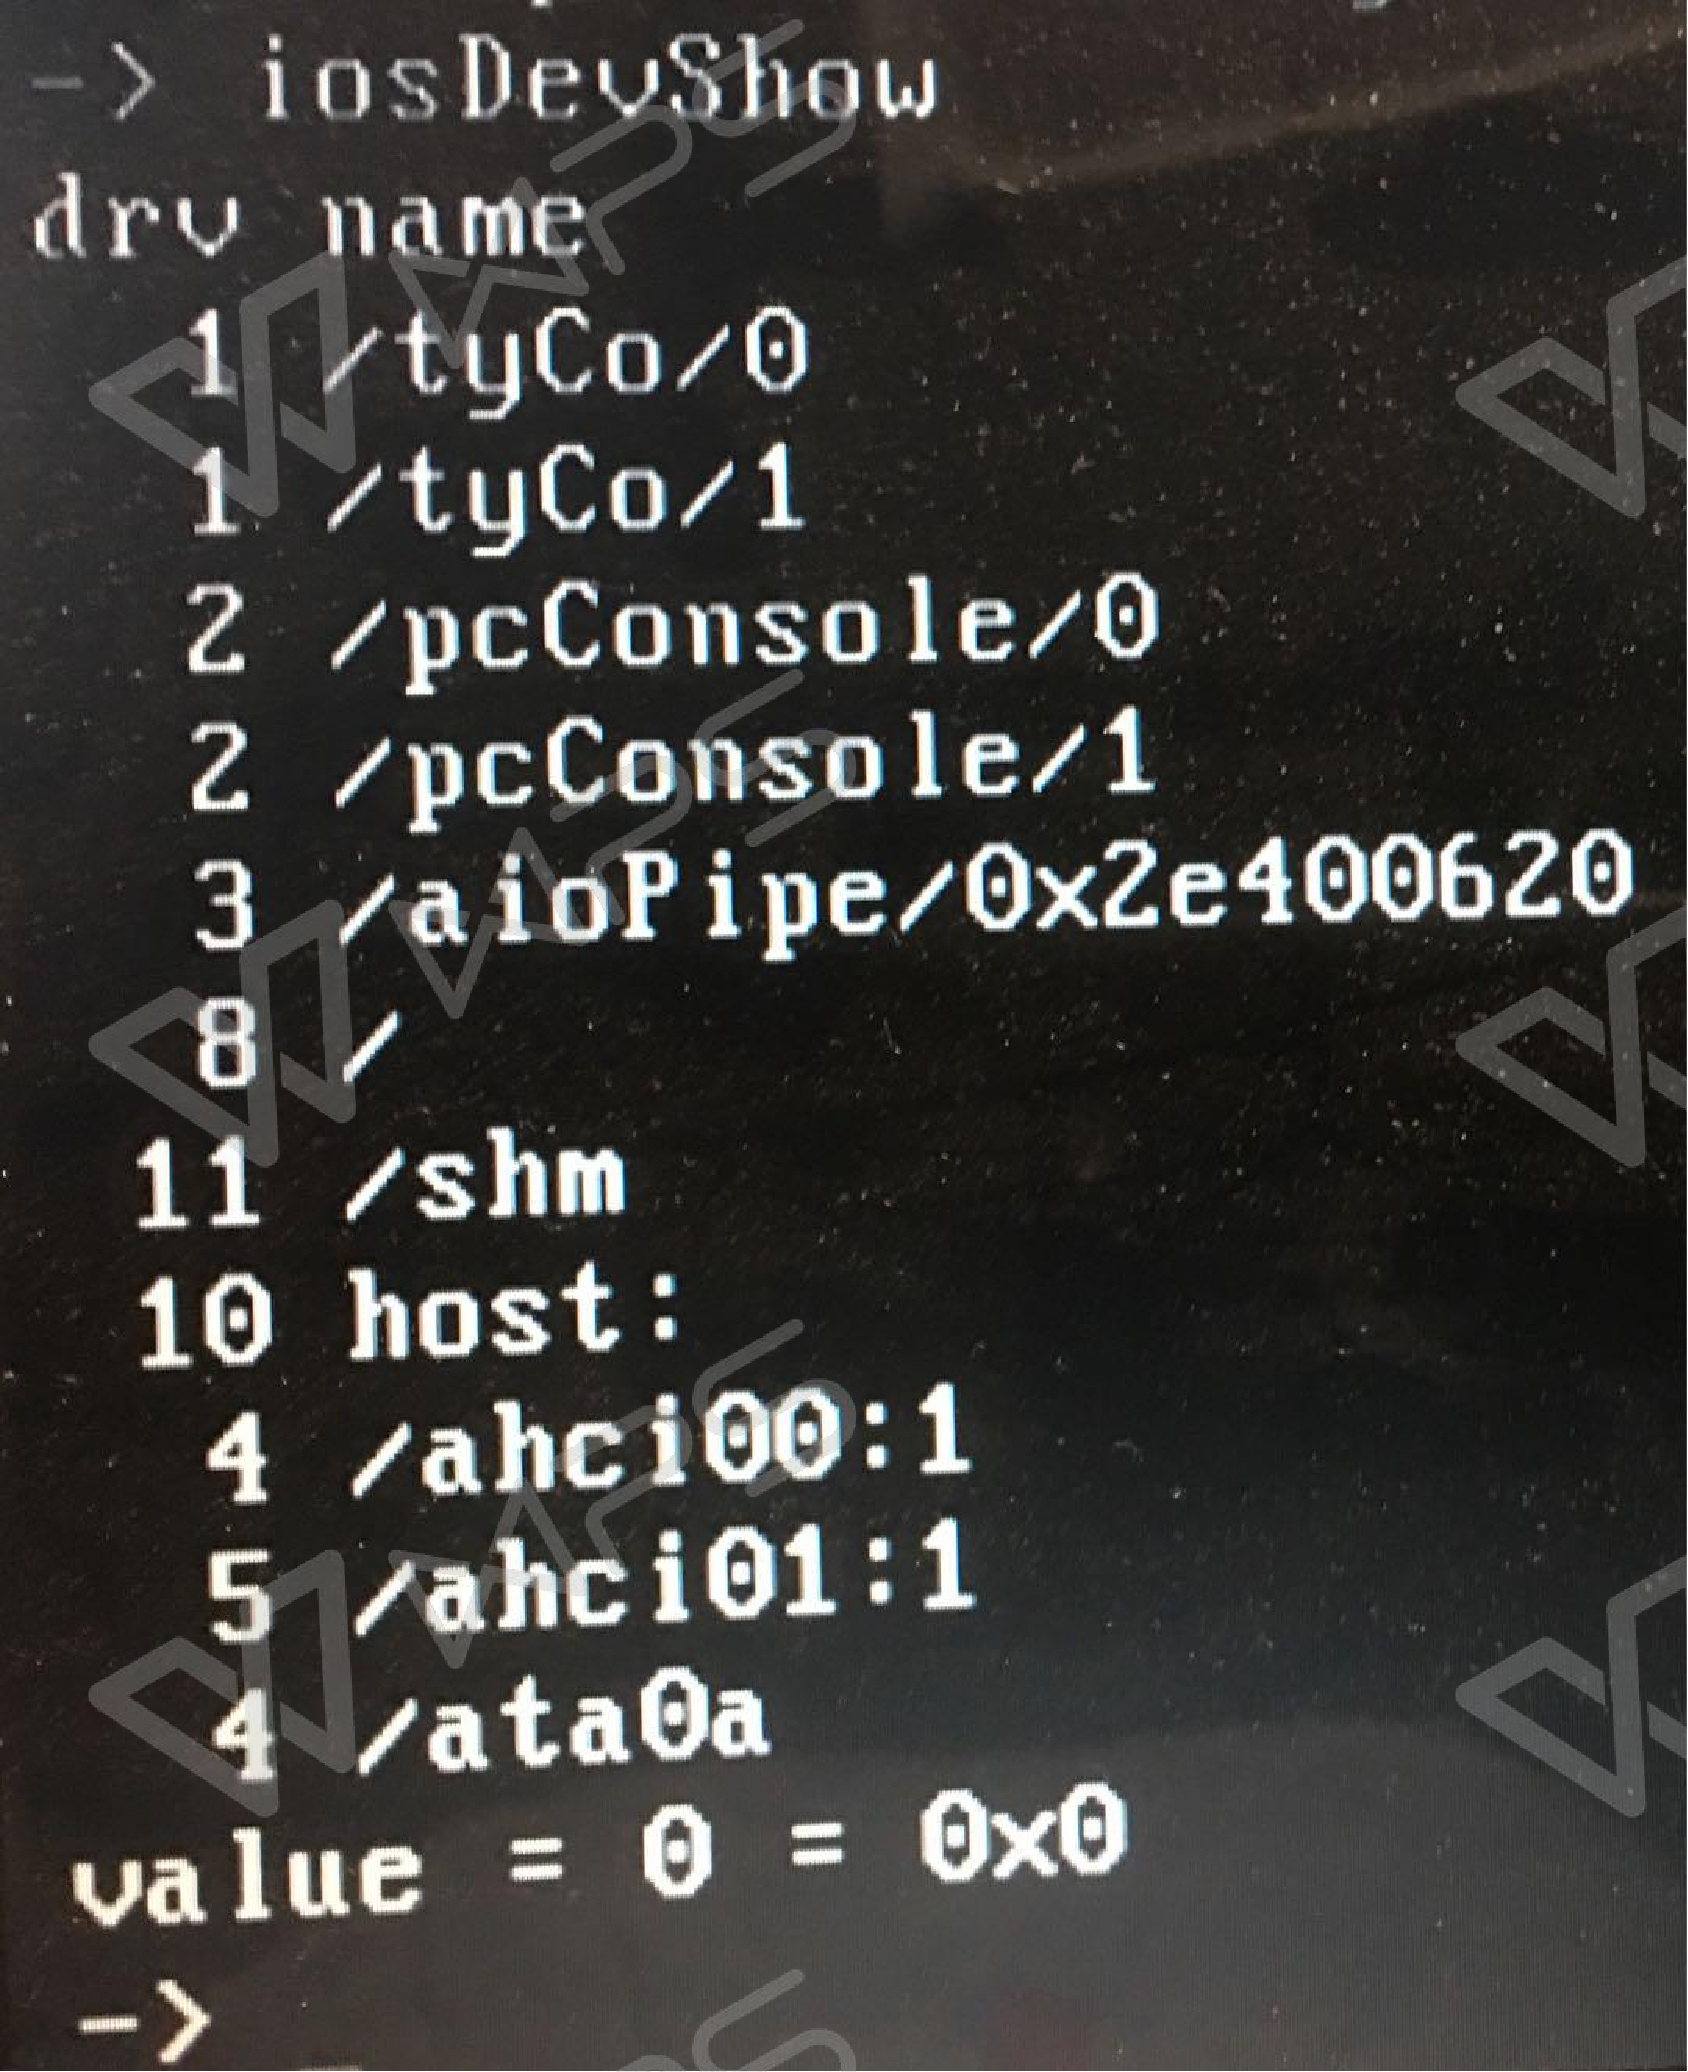
\includegraphics[width=0.7\textwidth ,height = 0.4\textwidth]{./graphics/iosDevShow.pdf}
\caption{驱动加载前系统设备表}\label{fig:iosDevShow}
\end{figure}

\begin{figure}[h]
\centering
  \begin{subfigure}[b]{0.4\textwidth}
  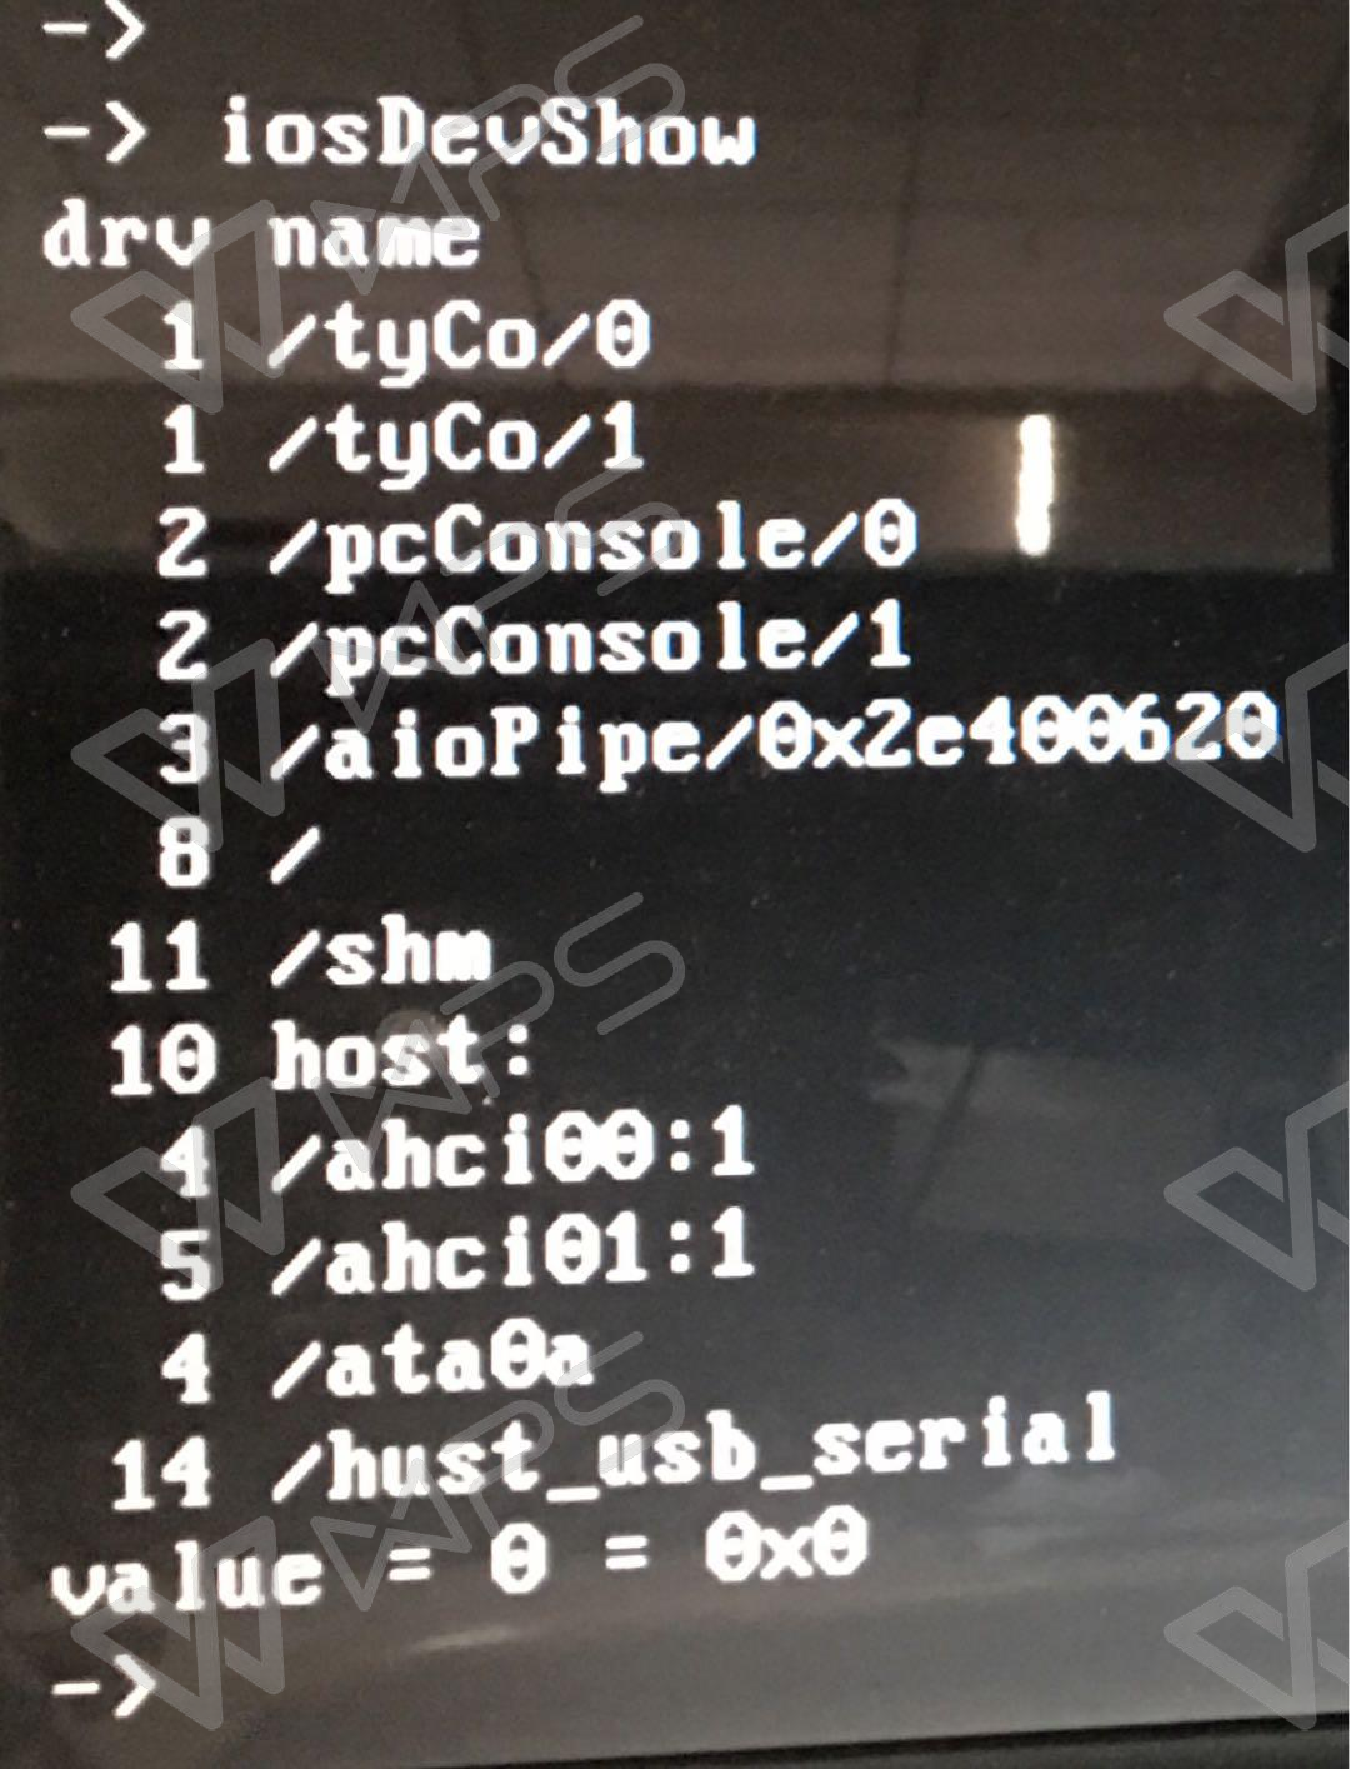
\includegraphics[width=\textwidth]{./graphics/iosDevShowS.pdf}
  \caption{单设备驱动}
  \end{subfigure}
  ~
  \begin{subfigure}[b]{0.4\textwidth}
  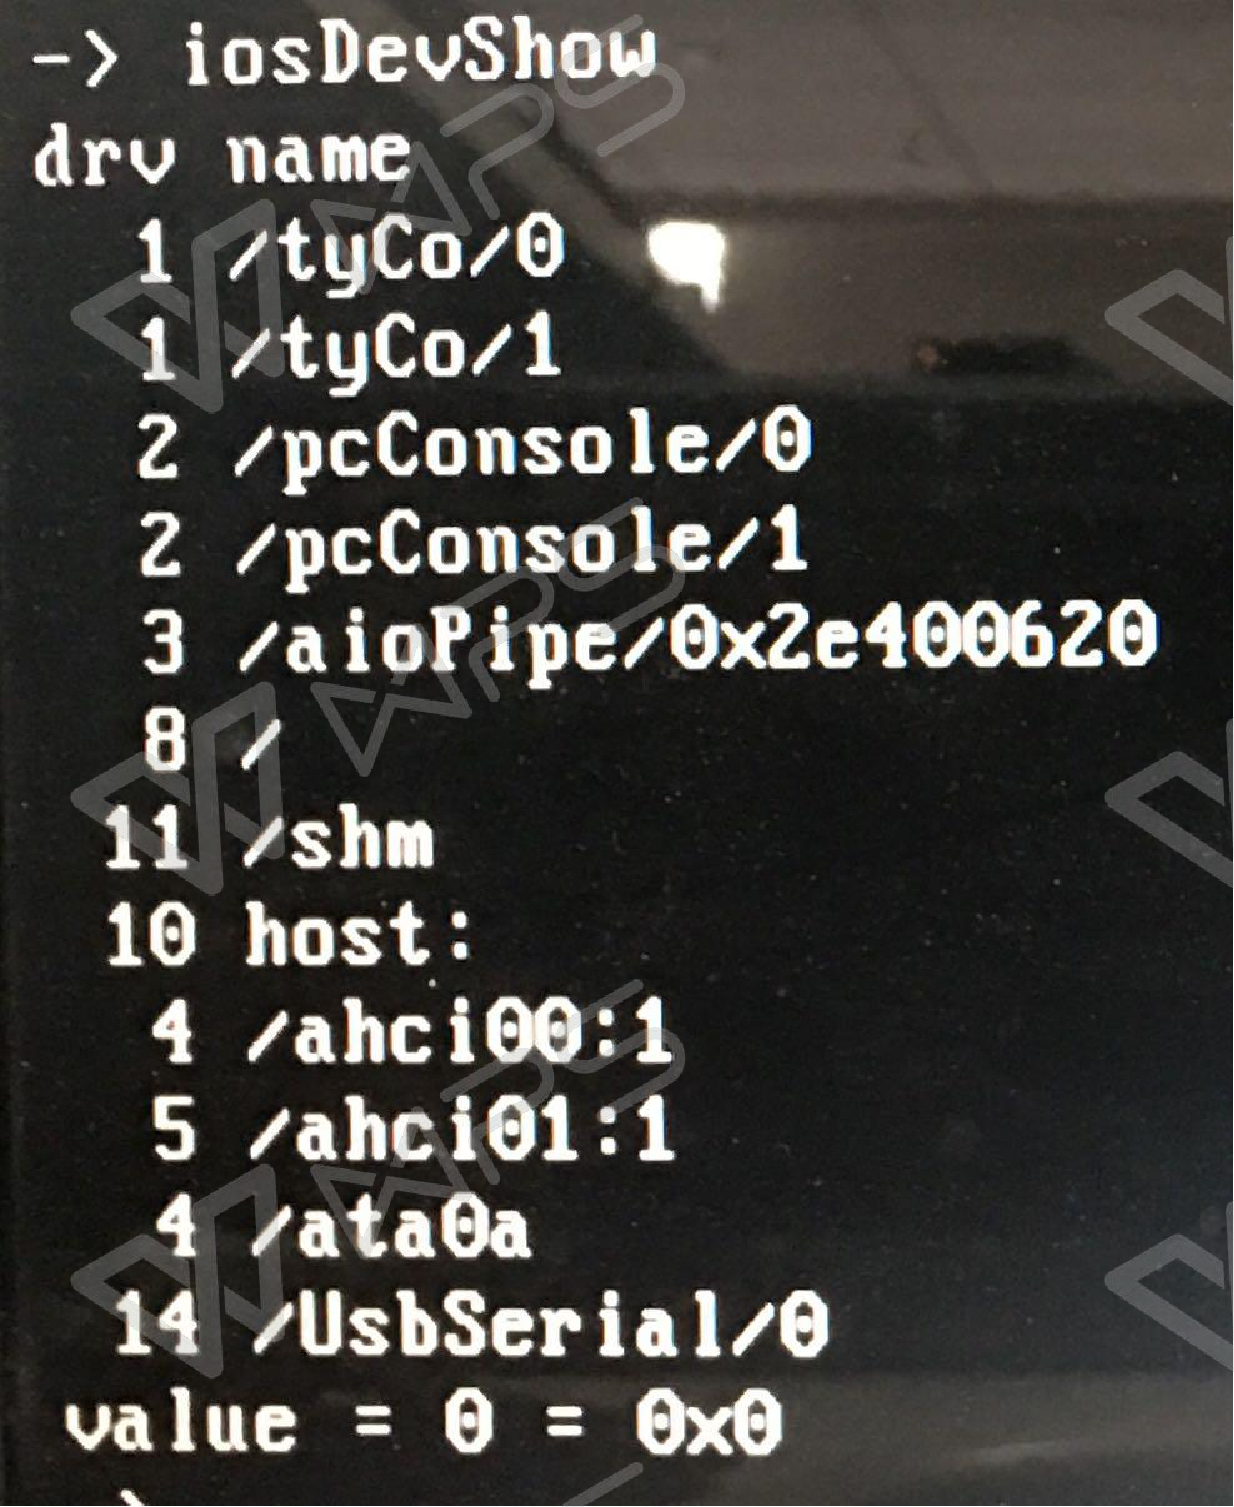
\includegraphics[width=\textwidth]{./graphics/iosDevShowM.pdf}
  \caption{多设备驱动}
  \end{subfigure}
\caption{驱动加载后系统设备表}\label{fig:加载驱动后系统上的设备表}
\end{figure}

\noindent 接下来查看设备驱动的接口是否已添加到驱动程序的列表当中,驱动加载前的系统驱动表如\autoref{fig:iosDrvShow}所示,驱动加载后的系统设备如\autoref{fig:加载驱动后系统上的驱动表}所示。
\begin{figure}[!h]
\centering
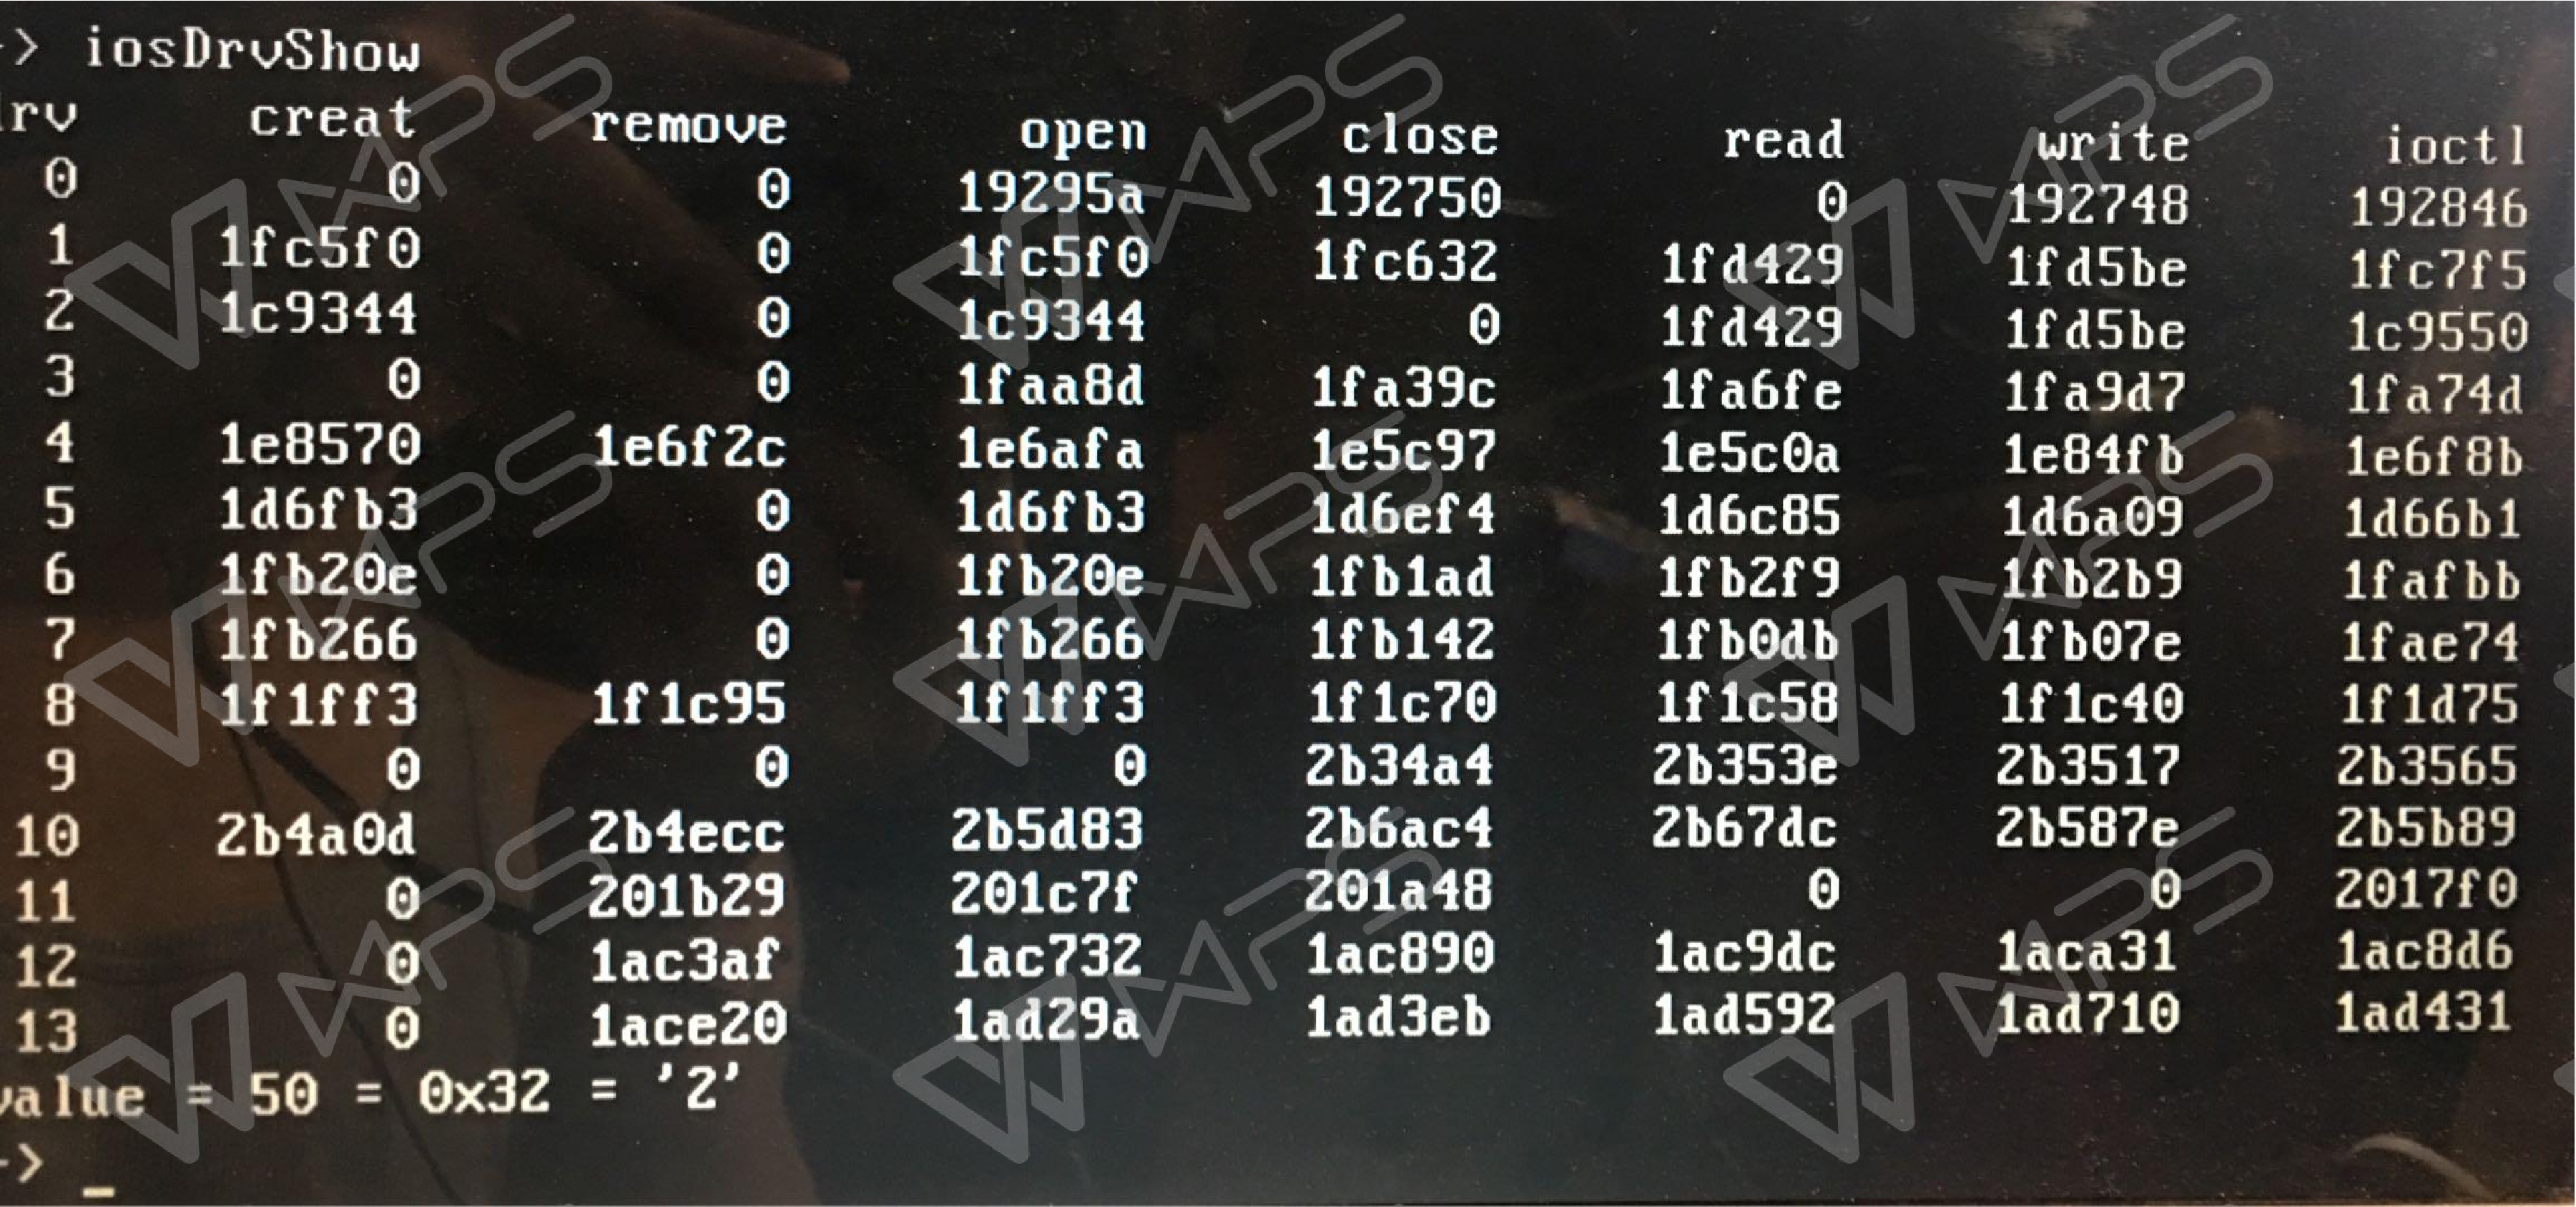
\includegraphics[width=.9\textwidth]{./graphics/iosDrvShow.pdf}
\caption{驱动加载前系统驱动表}\label{fig:iosDrvShow}
\end{figure}


\begin{figure}[h]
\centering
  \begin{subfigure}[b]{0.7\textwidth}
  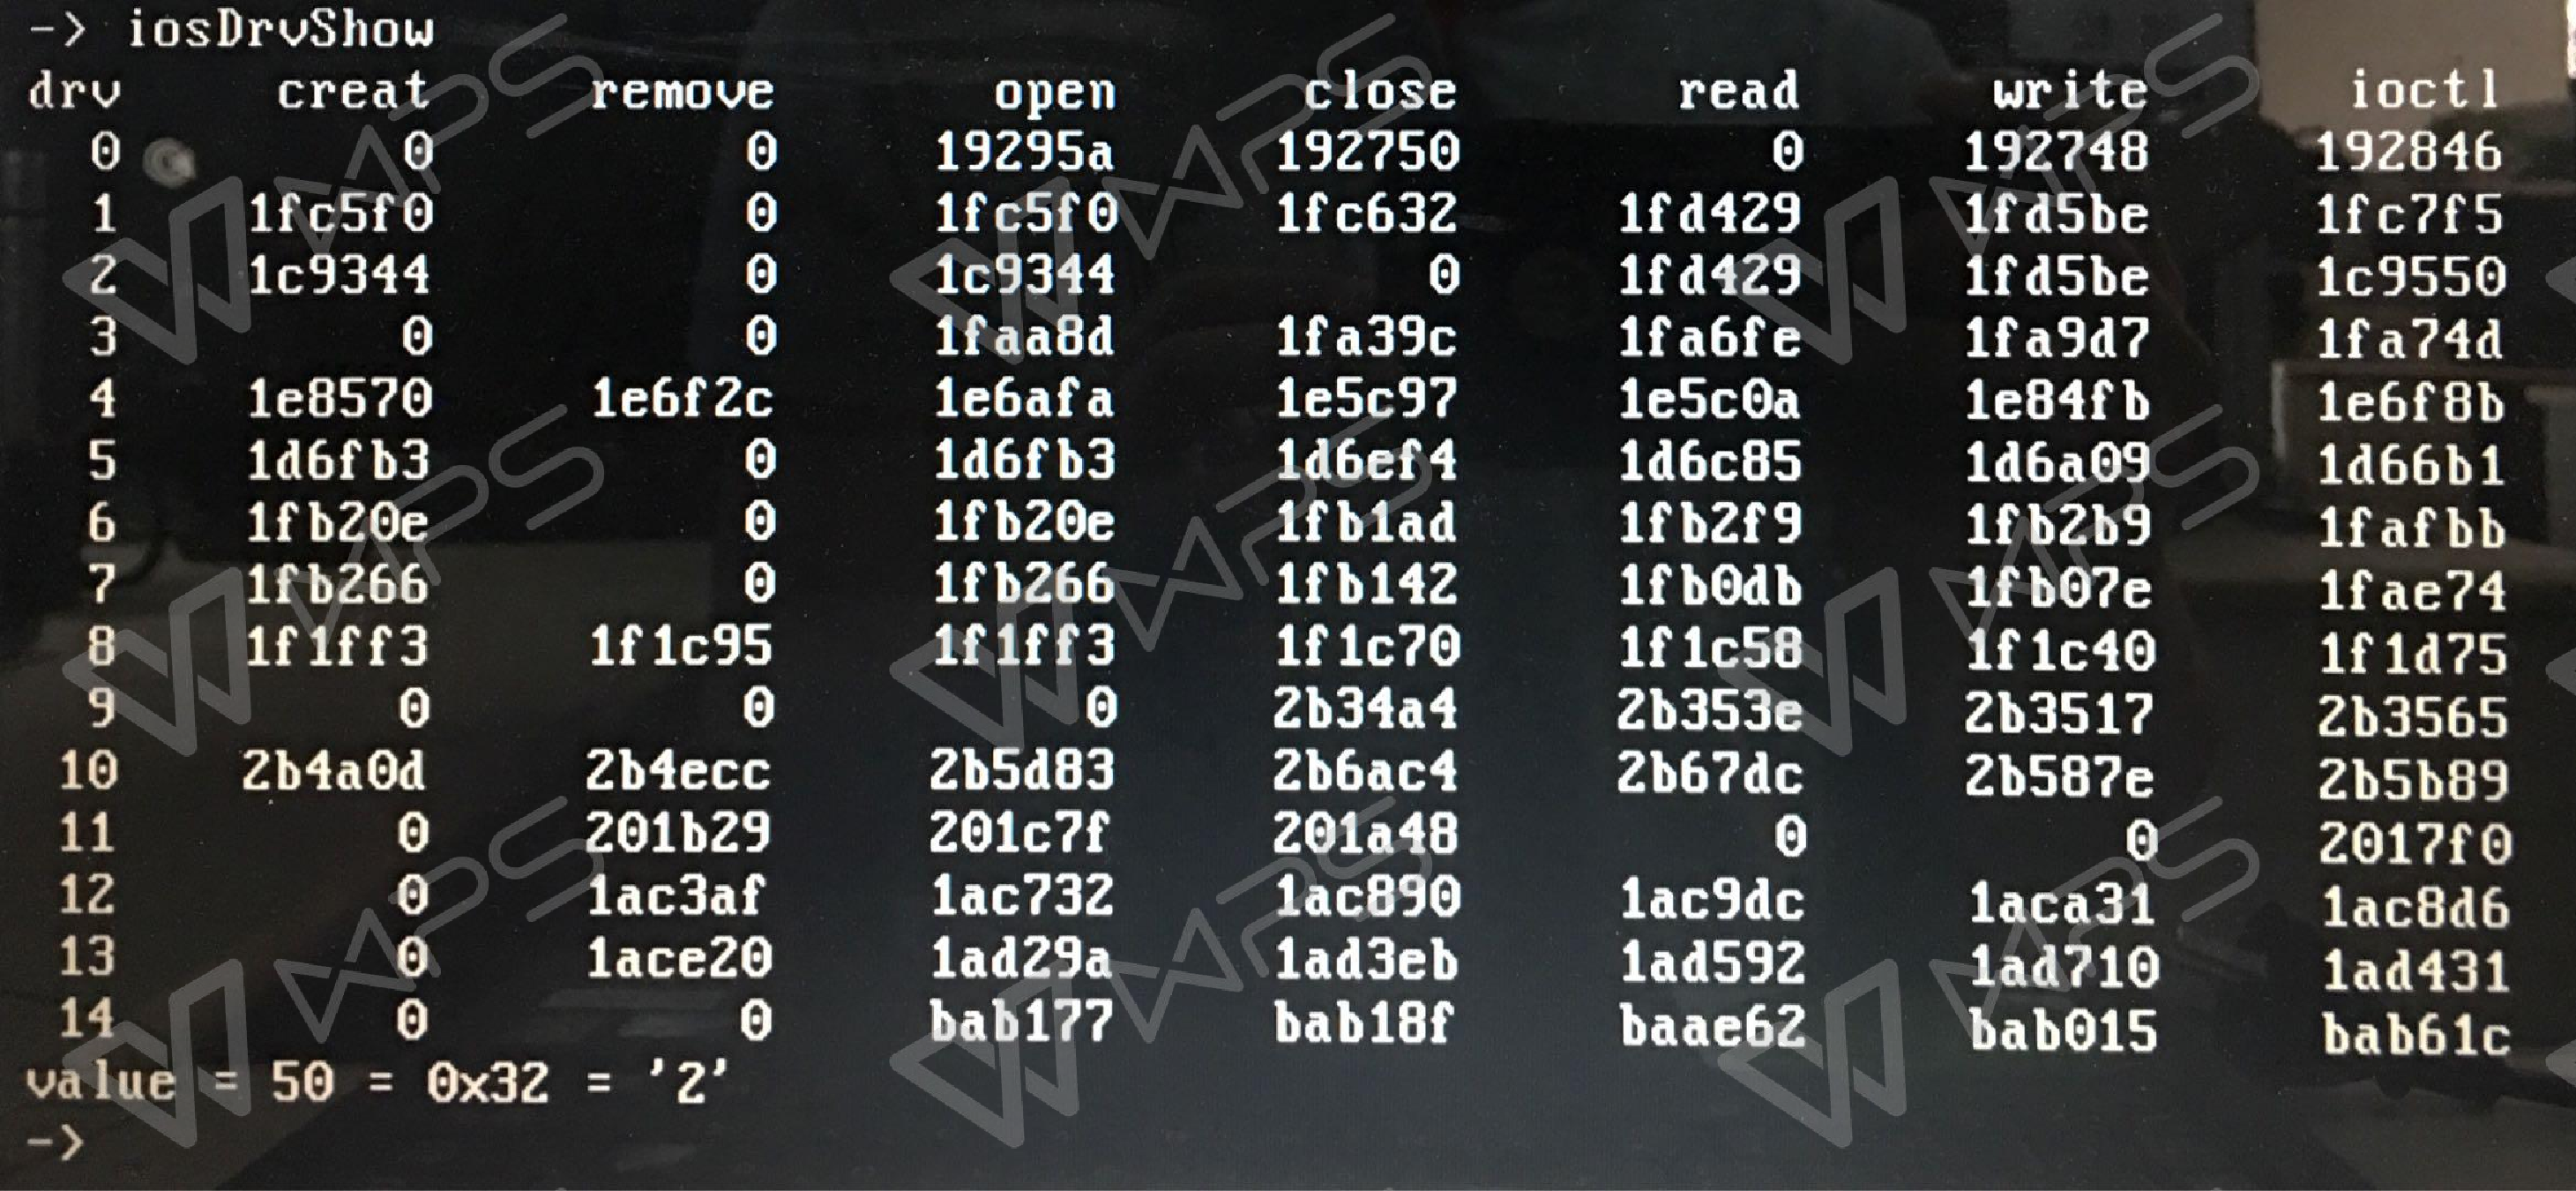
\includegraphics[width=\textwidth]{./graphics/iosDrvShowS.pdf}
  \caption{单设备驱动}
  \end{subfigure}
  ~
  \begin{subfigure}[b]{0.7\textwidth}
  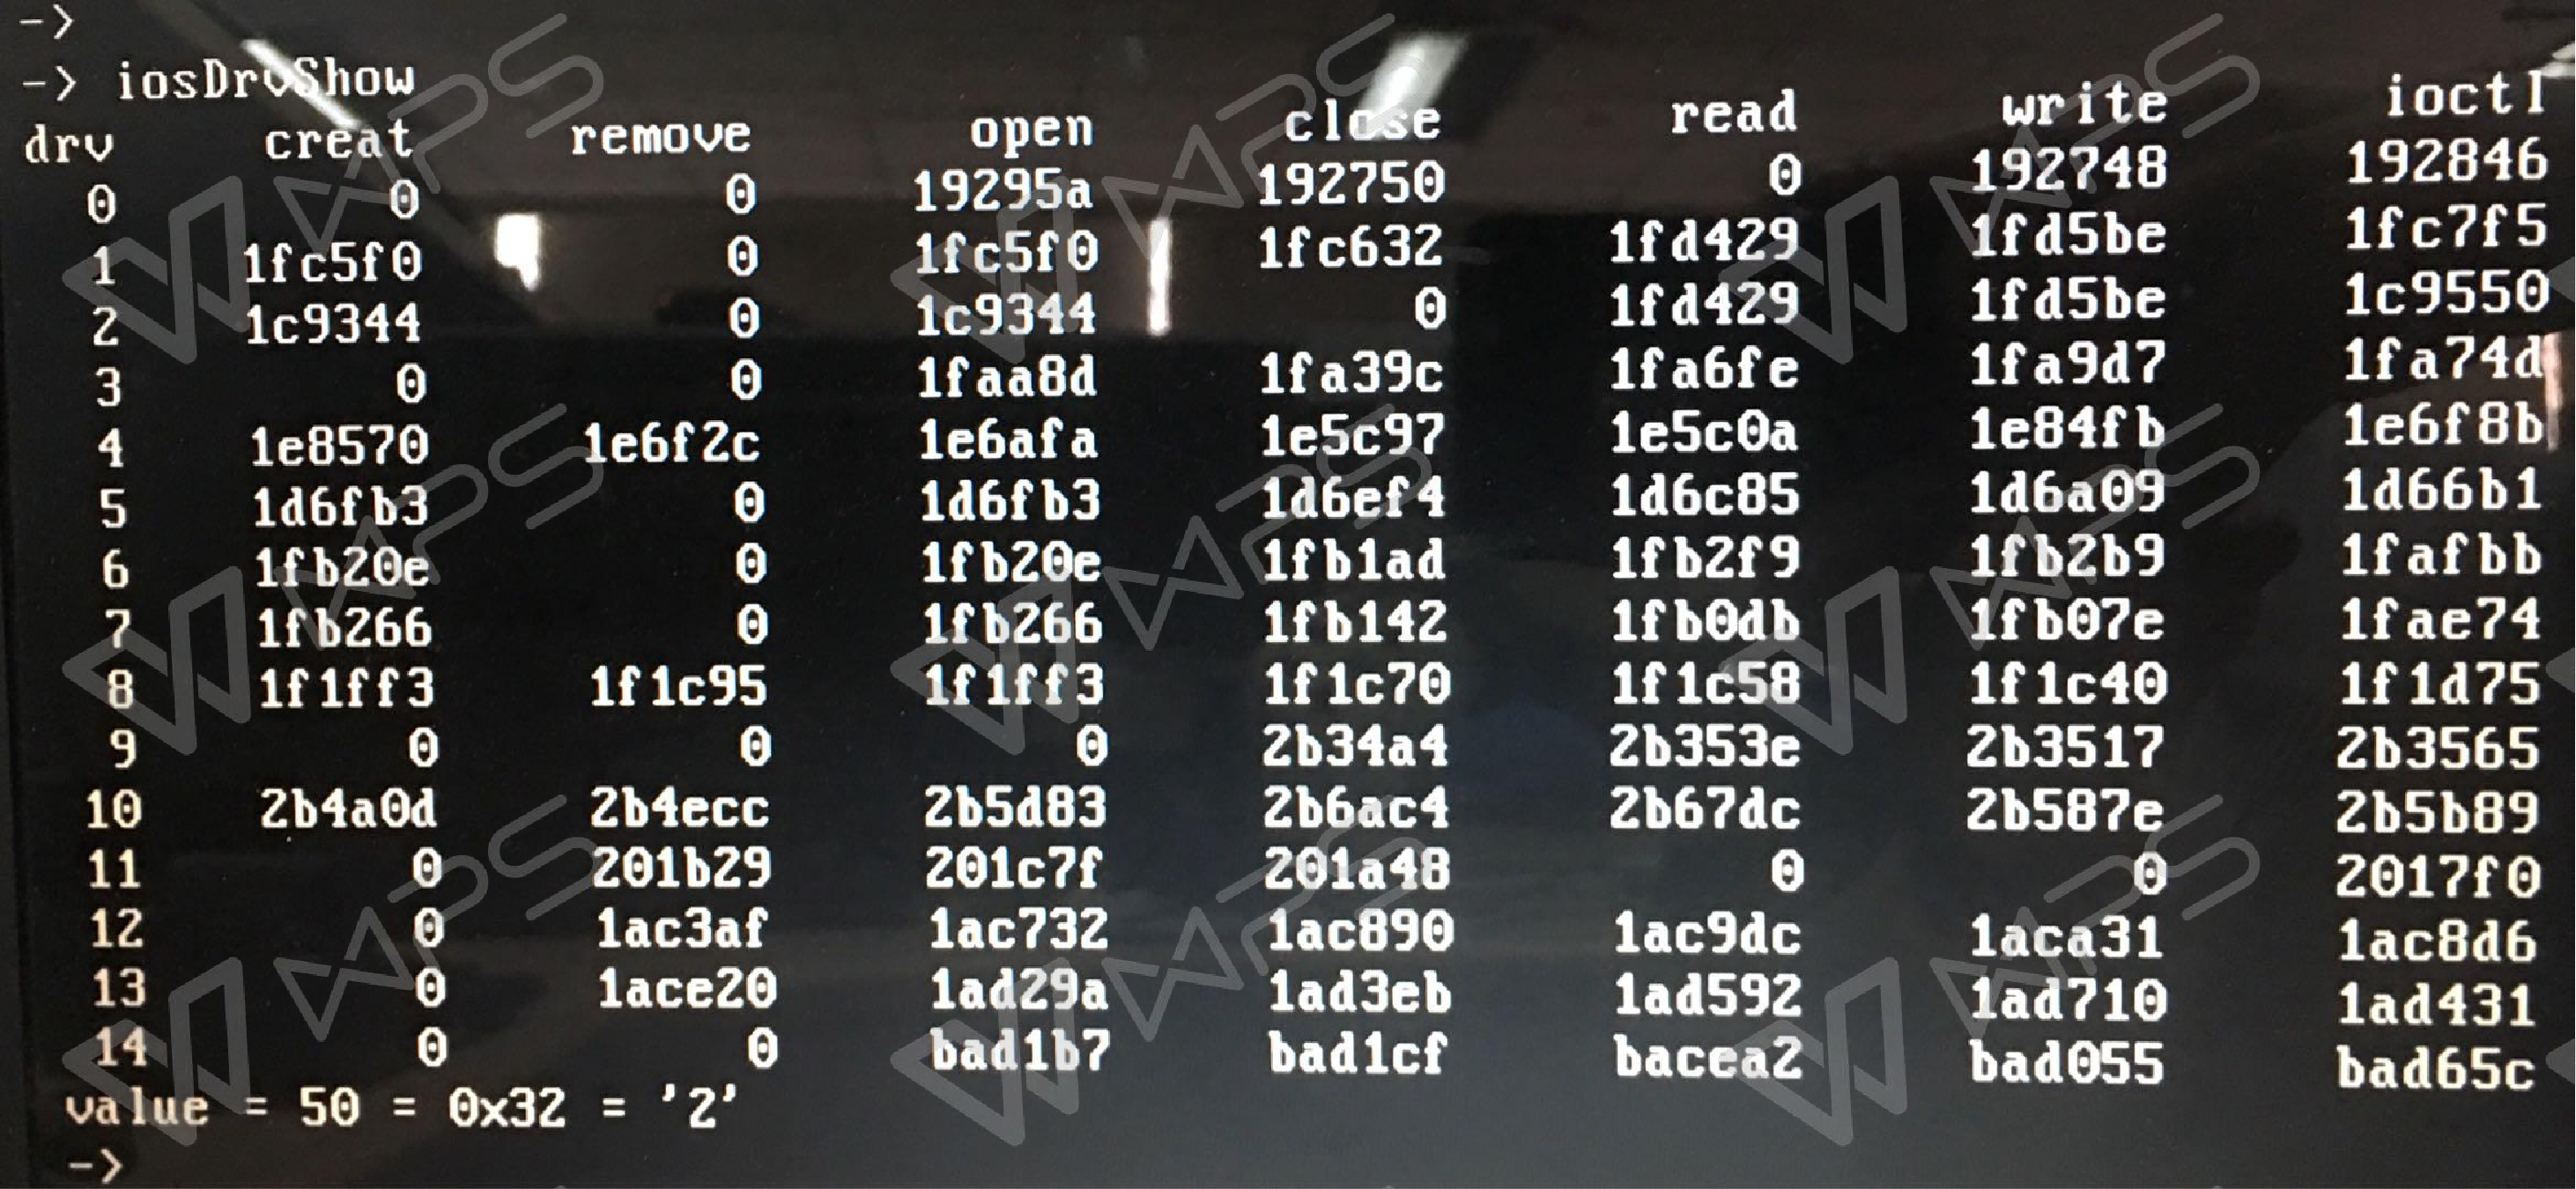
\includegraphics[width=\textwidth]{./graphics/iosDrvShowM.pdf}
  \caption{多设备驱动}
  \end{subfigure}
\caption{驱动加载系统驱动表}\label{fig:加载驱动后系统上的驱动表}
\end{figure}

\noindent 最后查看一下加载驱动之后是否能够正常的打开设备,打开设备之后应该会将其加入到系统文件描述符表当中,驱动加载前的文件描述符表如\autoref{fig:iosFdShow}所示,驱动加载后的文件描述符 表如\autoref{fig:加载驱动后系统上的文件描述符表}所示。
\begin{figure}[!h]
\centering
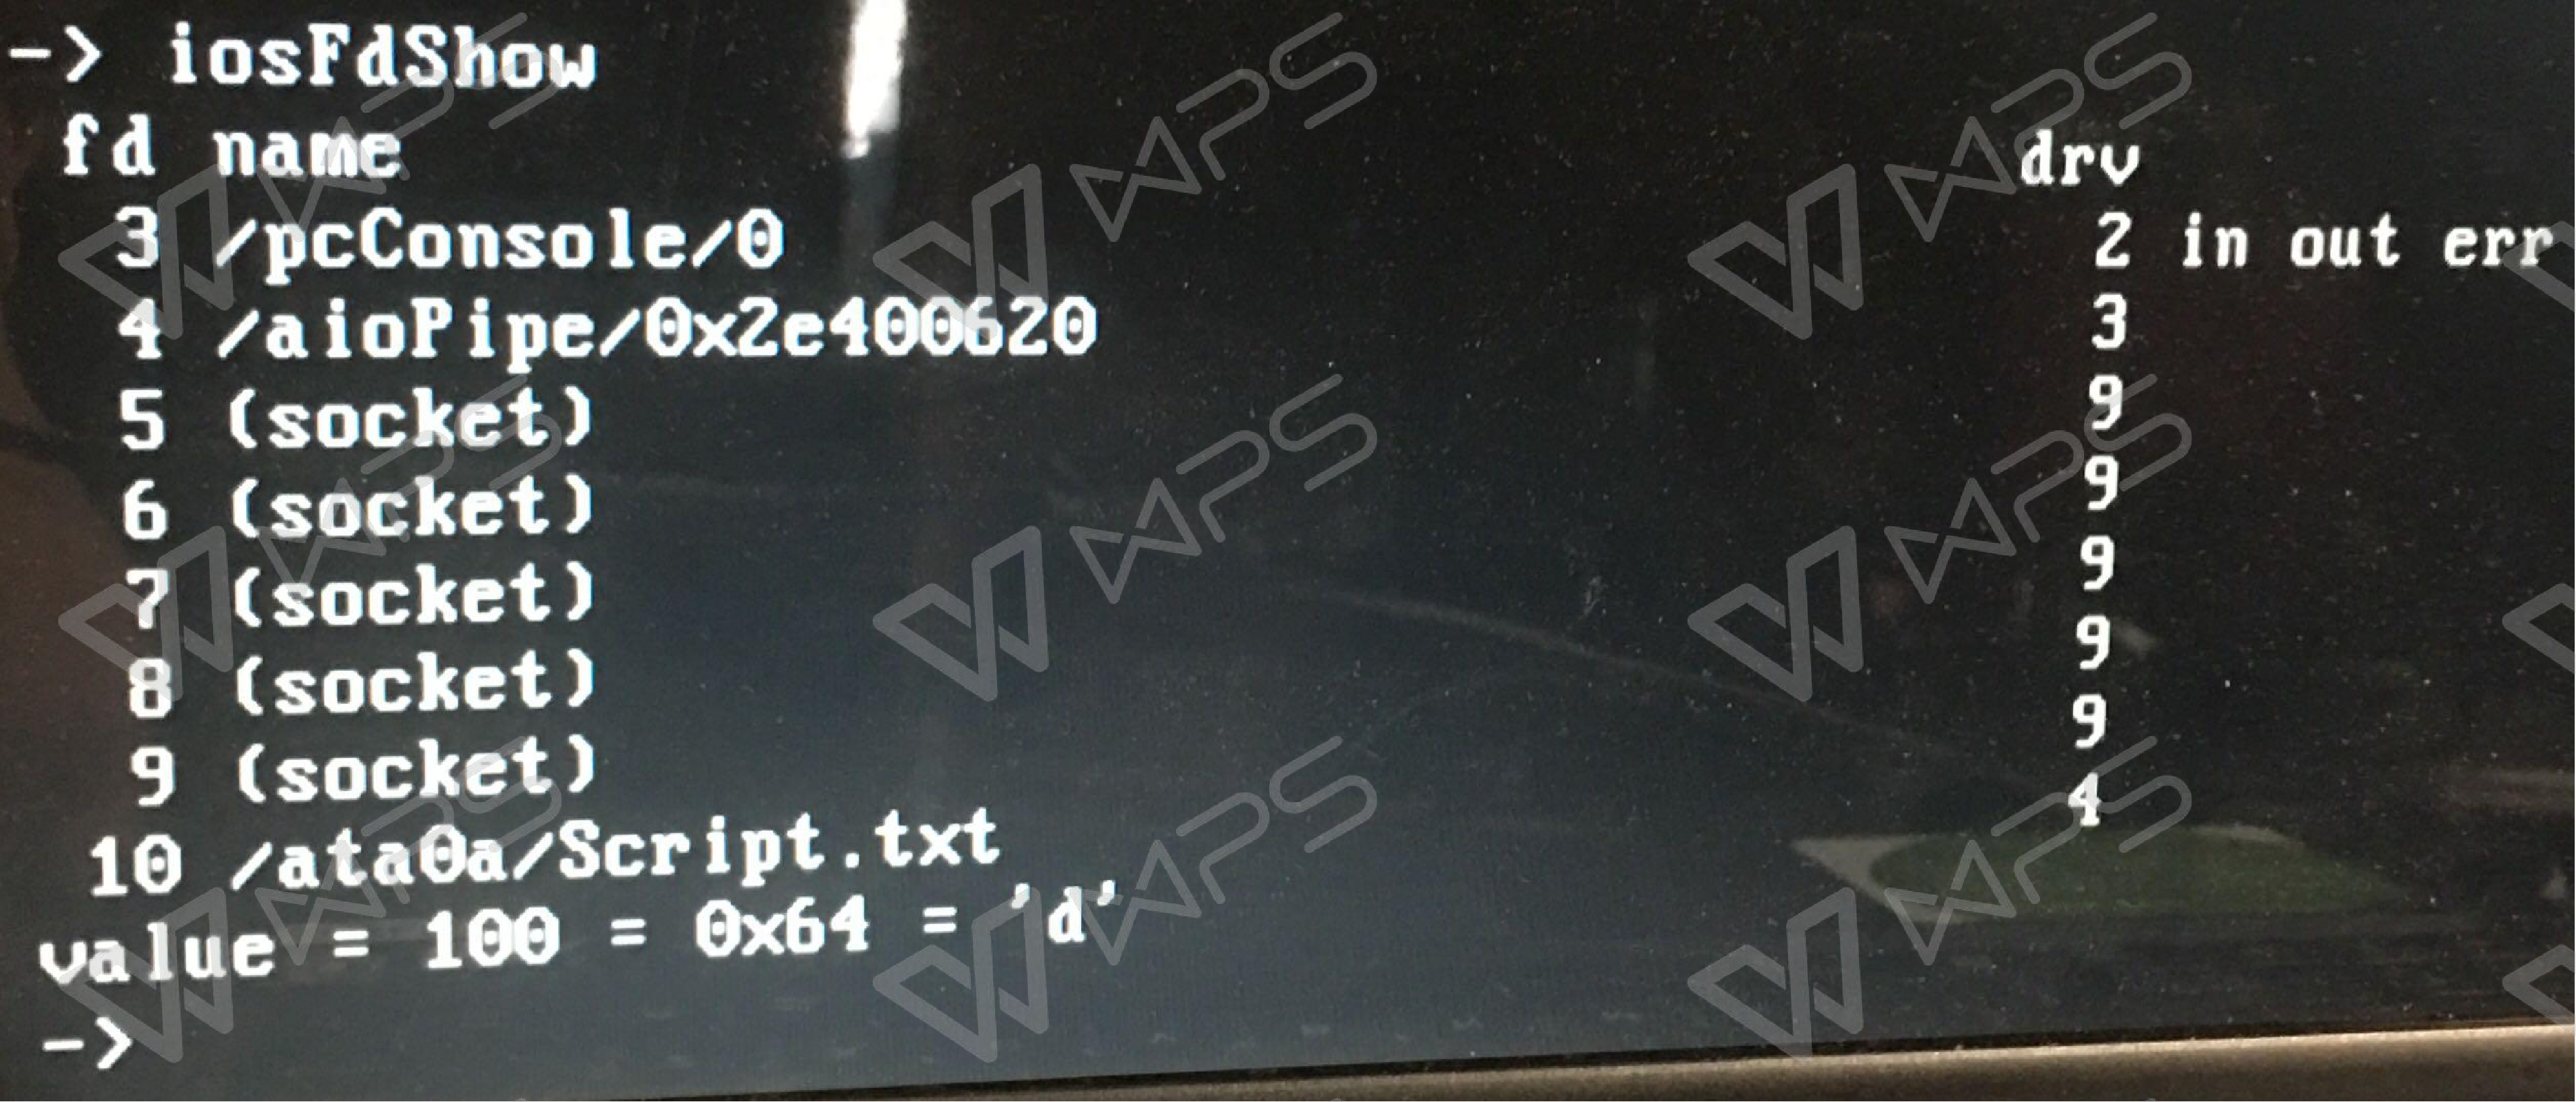
\includegraphics[width=.9\textwidth]{./graphics/iosFdShow.pdf}
\caption{当前系统上的文件描述符表}\label{fig:iosFdShow}
\end{figure}

\begin{figure}[h]
\centering
  \begin{subfigure}[b]{0.4\textwidth}
  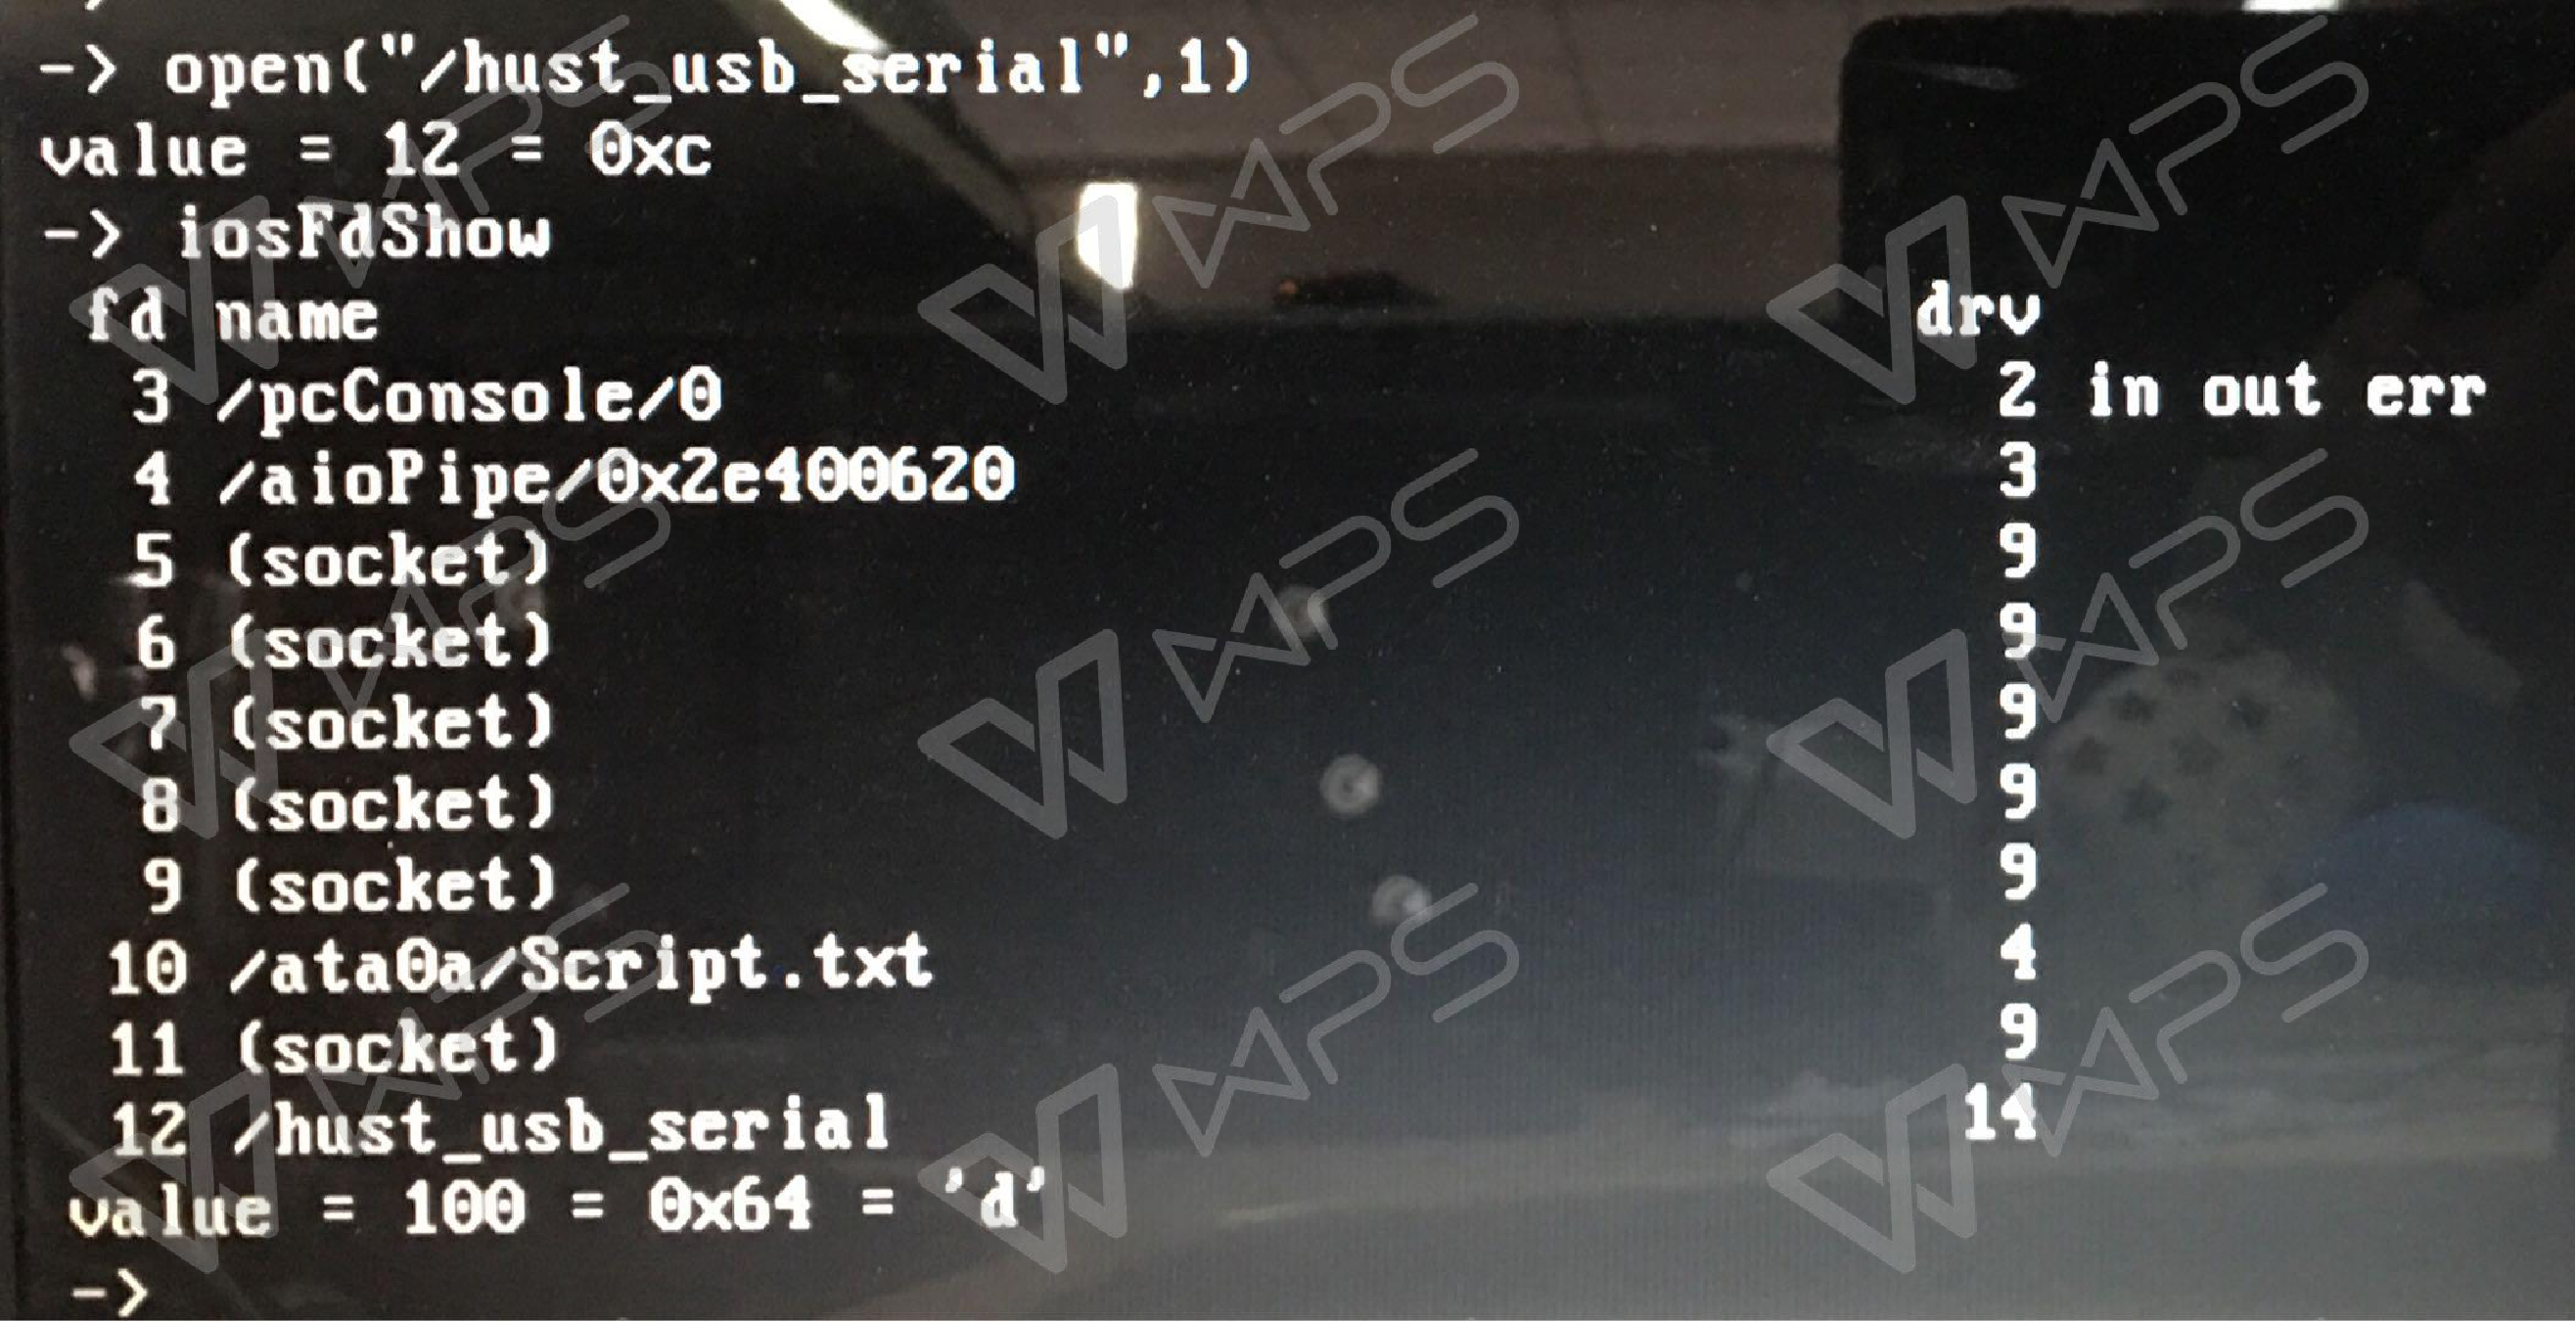
\includegraphics[width=\textwidth]{./graphics/iosFdShowS.pdf}
  \caption{单设备驱动}
  \end{subfigure}
  ~
  \begin{subfigure}[b]{0.4\textwidth}
  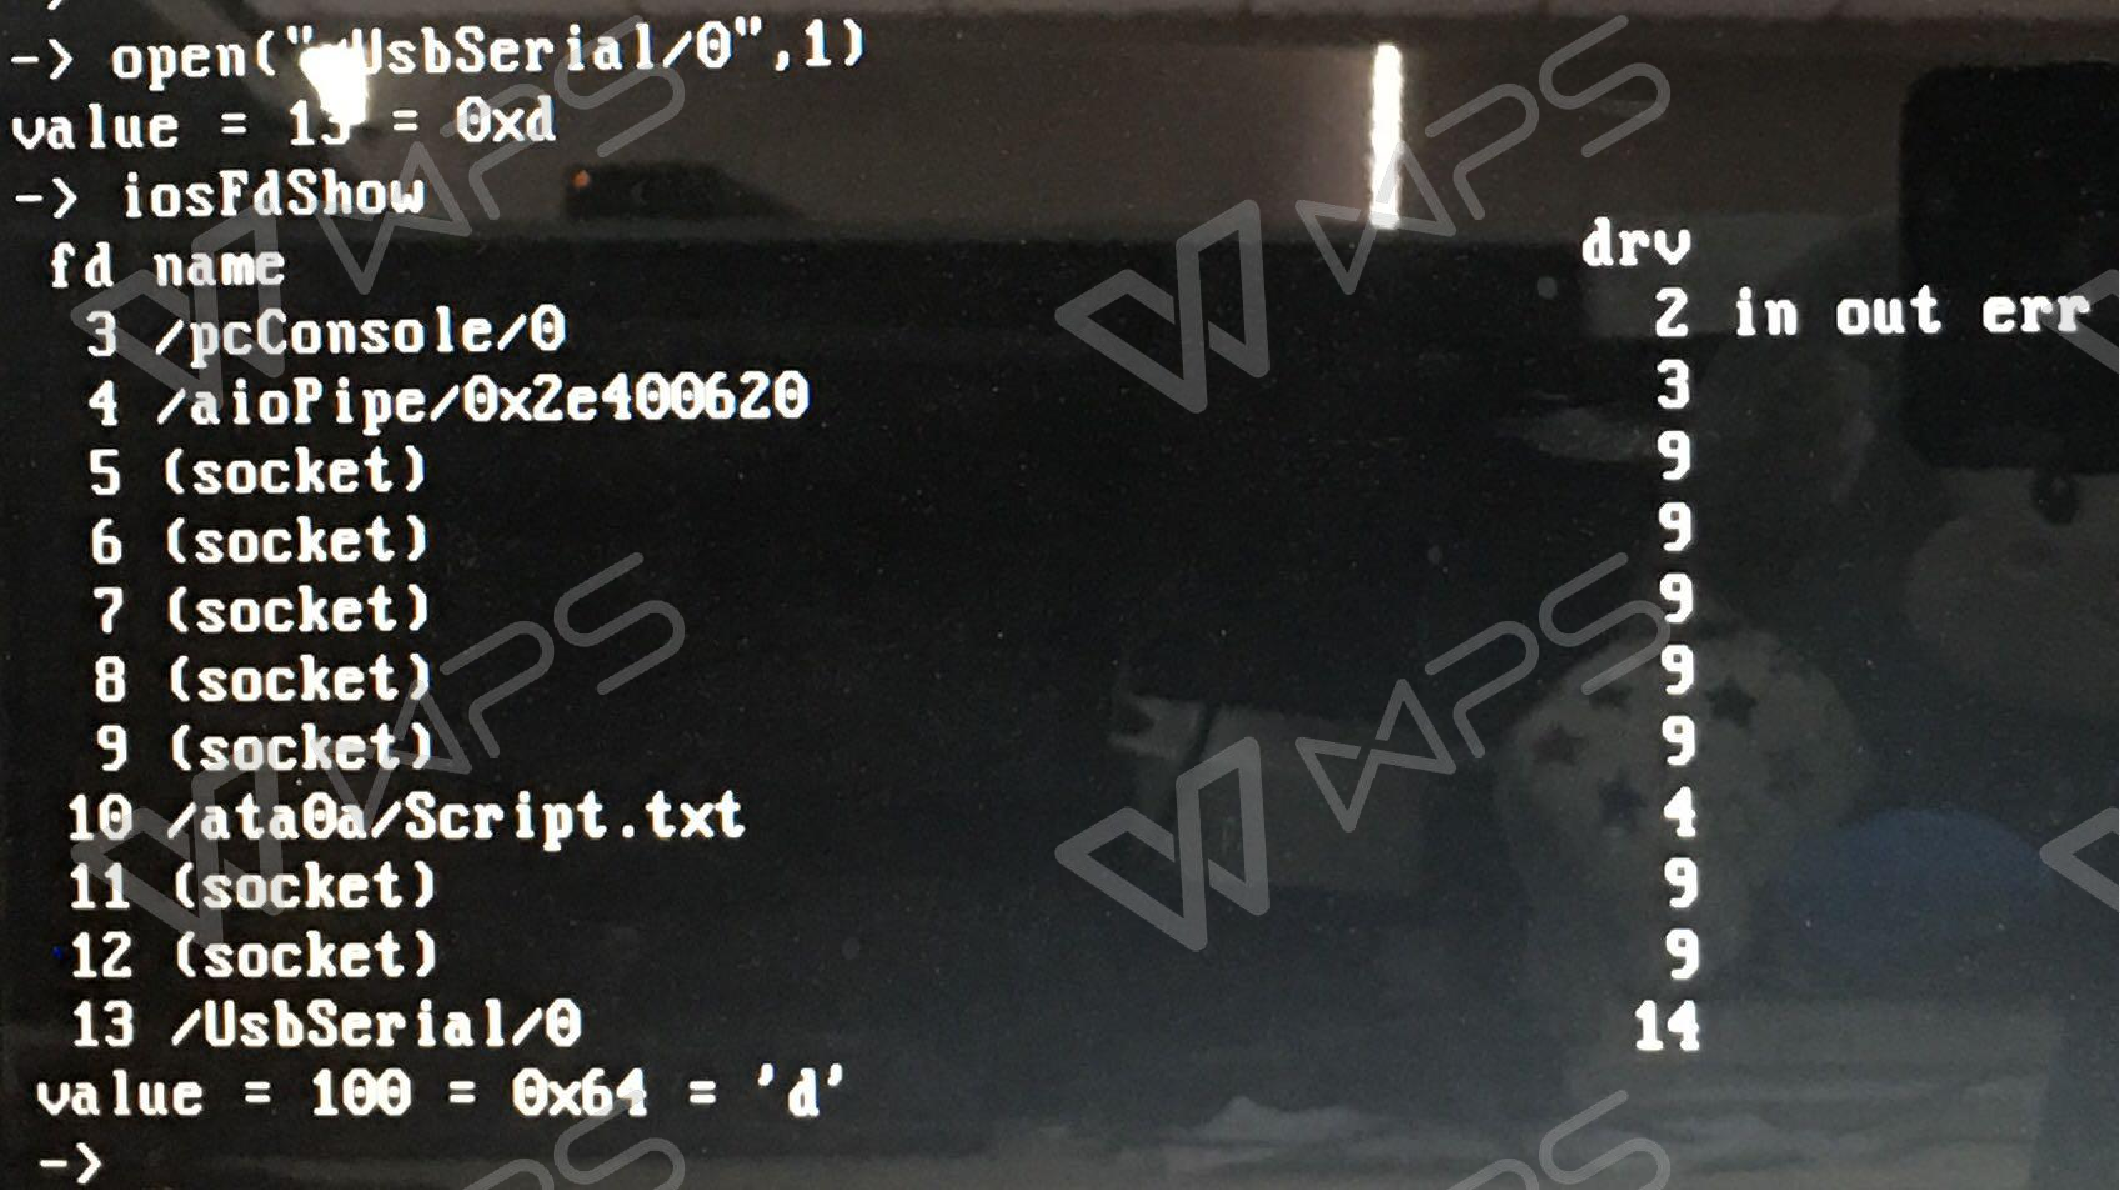
\includegraphics[width=\textwidth]{./graphics/iosFdShowM.pdf}
  \caption{多设备驱动}
  \end{subfigure}
\caption{加载驱动后系统上的文件名文件描述符表}\label{fig:加载驱动后系统上的文件描述符表}
\end{figure}

通过以上的验证说明了驱动程序已经被正常的安装,标准系统IO接口和驱动程序的IO子系统已经挂接成功。下一步将要进行进一步的功能测试,检测内部的各个IO接口是否能够正常的完成工作。
	
\section{驱动程序读写测试}
	驱动通常会作为操作系统内核的一部分来实现,即便现在很多系统支持驱动的动态加载,但是驱动代码在执行时,依然是以内核代码模式进行执行的,所以如果驱动程序存在 BUG,会导致操作系统的崩溃。所以调试驱动是一项十分关键的工作,必须对驱动进行仔细检查,并需要经受长时间运行考验,其调试过程同时也是对硬件和驱动进行验证的过程。
	由于VxWorks同时存在RTP模式和task模式,所以在这两种模式下都需要进行读写测试。
测试条件: 装有我们编写的USB口转串口驱动的VxWorks PC机,装有串口调试工具的windows PC机,USB转TTL模块在两台PC之间进行数据传输。

\subsection{RTP模式下的读写测试}
	测试报告如\autoref{tab:RTP模式下串口测试}所示。
\begin{table}[!h]
\centering
\begin{tabular}{|c|c|c|c|c|c|c|c|}
\hline
{\hei{波特率}} & {\hei{数据位}} & {\hei{数据位}} & {\hei{数据方向}} &{\hei{发送周期} & {\hei{发送次数}} &{\hei{信息数量}} &{\hei{正确率}} \\ 
\hline
{9600} & {8} & {0} & {读} & {0.1S/次} & {10000} & {500单词/次} & {100\%}\\
\hline
{9600} & {8} & {0} & {写} & {0.1S/次} & {10000} & {500单词/次} & {100\%}\\
\hline
{9600} & {8} & {0} & {读\& 写} & {0.1S/次} & {10000} & {500单词/次} & {100\%}\\
\hline 
{115200} & {8} & {0} & {读} & {0.1S/次} & {10000} & {500单词/次} & {100\%}\\
\hline
{115200} & {8} & {0} & {写} & {0.1S/次} & {10000} & {500单词/次} & {100\%}\\
\hline
{115200} & {8} & {0} & {读\& 写} & {0.1S/次} & {10000} & {500单词/次} & {100\%}\\
\hline
{921600} & {8} & {0} & {读} & {0.1S/次} & {10000} & {500单词/次} & {99.8\%}\\
\hline
{921600} & {8} & {0} & {写} & {0.1S/次} & {10000} & {500单词/次} & {100\%}\\
\hline
{921600} & {8} & {0} & {读\& 写} & {0.1S/次} & {10000} & {500单词/次} & {99.2\%}\\
\hline
\end{tabular}
\caption{RTP模式下串口测试}\label{tab:RTP模式下串口测试}
\end{table}


\subsection{task模式下的读写测试}
测试报告如\autoref{tab:task模式下串口测试}所示。
\begin{table}[!h]
\centering
\begin{tabular}{|c|c|c|c|c|c|c|c|}
\hline
{\hei{波特率}} & {\hei{数据位}} & {\hei{数据位}} & {\hei{数据方向}} &{\hei{发送周期} & {\hei{发送次数}} &{\hei{信息数量}} &{\hei{正确率}} \\ 
\hline
{9600} & {8} & {0} & {读} & {0.1S/次} & {10000} & {500单词/次} & {100\%}\\
\hline
{9600} & {8} & {0} & {写} & {0.1S/次} & {10000} & {500单词/次} & {100\%}\\
\hline
{9600} & {8} & {0} & {读\& 写} & {0.1S/次} & {10000} & {500单词/次} & {100\%}\\
\hline 
{115200} & {8} & {0} & {读} & {0.1S/次} & {10000} & {500单词/次} & {100\%}\\
\hline
{115200} & {8} & {0} & {写} & {0.1S/次} & {10000} & {500单词/次} & {100\%}\\
\hline
{115200} & {8} & {0} & {读\& 写} & {0.1S/次} & {10000} & {500单词/次} & {100\%}\\
\hline
{921600} & {8} & {0} & {读} & {0.1S/次} & {10000} & {500单词/次} & {100\%}\\
\hline
{921600} & {8} & {0} & {写} & {0.1S/次} & {10000} & {500单词/次} & {100\%}\\
\hline
{921600} & {8} & {0} & {读\& 写} & {0.1S/次} & {10000} & {500单词/次} & {99.6\%}\\
\hline
\end{tabular}
\caption{task模式下串口测试}\label{tab:task模式下串口测试}
\end{table}

在两种模式下都出现了在波特率较高的时候出现误码的现象,尤其是在同时进行数据的收发的时候出现误码的概率更大。会有很多的原因导致串口出现误码,例如干扰、接地不好、数据率过高、双方定时不一致等都会导致误码率的升高。

\section{应用程序接口测试}
\subsection{标准输出重定向测试}
测试条件:装有我们编写的USB口转串口驱动的VxWorks PC机,封装好的标准输出重定向接口, 
装有串口调试工具的windows PC机,USB转TTL模块在两台PC之间进行数据传输。

测试同样分为RTP模式和task模式,在两种模式下实现重定向的机制并不一样。
1. task模式:

	在VxWorks中启动一个task程序,先调用标准输出重定向接口,查看其是否能够在程序中将标准输出重定向到串口.再定向回来。循环进行下去,查看输出是否正确。简单的测试程序如下:
\lstset{language=C}
\begin{lstlisting}
void test1(void)
{
	int j =0;
	while(j < 10000){
		ResetStdOut(1);
		printf("<task printf test:> shold be in windows\n");		
		ResetStdOut(0);
		printf("<task printf test:> shold be in VxWorks\n");
	}
}
\end{lstlisting}
测试结果显示重定向接口能够在task模式下完美的完成重定向的功能。

2. RTP模式:
	
	RTP模式下的测试方式与在task模式下一样,在VxWorks中启动一个RTP程序,先调用标准输出重定向接口,查看其是否能够在程序中将标准输出重定向到串口.再定向回来,循环进行下去,查看输出是不是正确。简单的测试程序如下:
\lstset{language=C}
\begin{lstlisting}
int main()
{
	int j =0;
	while(j < 10000){
		ResetStdOut(1);
		printf("<RTP printf test:> shold be in windows\n");		
		ResetStdOut(0);
		printf("<RTP printf test:> shold be in VxWorks\n");
	}
}
\end{lstlisting}
注意这里的两个程序的区别,RTP模式下是main函数开始的,而task模式下是以内核模块的方式运行的。测试结果显示RTP模式下标准输出重定向也能够正常的完成工作,不会对系统造成混乱。

\subsection{Log日志接口测试}
	Log接口函数在RTP模式下和task模式下的实现方法是一样的,所以就不需要区分两种实现方式下的测试结果。我们以在RTP模式下的测试结果为例,测试完成的界面如\autoref{fig:RoutonLog}所示。在日志信息的显示框我们可以看到不同的颜色标识的不同级别的信息,包括我们自定义的协议的日志级别、进程号、进程名等信息都能正常的进行封装,并被正确的解析出来。
\begin{figure}[!h]
\centering
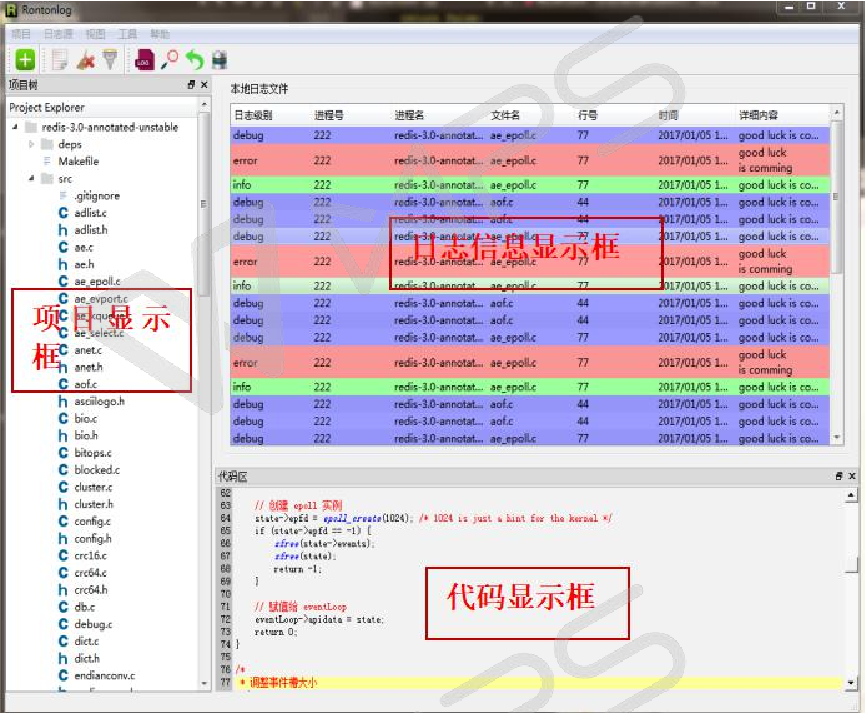
\includegraphics[width=1.0\textwidth]{./graphics/routonLogRun.pdf}
\caption{主机端日志分析工具测试界面}\label{fig:RoutonLog}
\end{figure}

测试报告如\autoref{tab:Log接口测试}所示。
\begin{table}[!h]
\centering
\begin{tabular}{|c|c|c|c|c|c|c|}
\hline
{\hei{波特率}} & {\hei{数据位}} & {\hei{数据位}} & {\hei{数据方向}}  & {\hei{发送次数}} &{\hei{信息类型}} &{\hei{正确率}} \\ 
\hline
{115200} & {8} & {0} & {写}  & {1000} & {LogE()} & {100\%}\\
\hline
{115200} & {8} & {0} & {写}  & {1000} & {LogW()} & {100\%}\\
\hline
{115200} & {8} & {0} & {写}  & {1000} & {LogI()} & {100\%}\\
\hline
{921600} & {8} & {0} & {写}  & {1000} & {LogO()} & {100\%}\\
\hline
{921600} & {8} & {0} & {写}  & {1000} & {LogD()} & {100\%}\\
\hline
\end{tabular}
\caption{Log接口测试}\label{tab:Log接口测试}
\end{table}

	需要注意的是上述的测试数据的是在1000次的循环内依次发送LogE、LogW、LogI、LogO、LogD的信息测试出来的,并不是每个级别的信息单独一个程序发送的。

